\chapter{中断怎样把设备和用户程序带进内核}

异常由当前指令引起，硬件中断则可能在任意指令之间到来。内核要从 PIC 接收
IRQ，保存被打断的现场，调用驱动，再发送 EOI。建立 TSS 和用户页表以后，
同一套入口还要安全处理 Ring 3 到 Ring 0 的特权切换。

\chapterroute{PIC、IRQ 和 IDT $\rightarrow$ 中断现场与嵌套边界
$\rightarrow$ 时钟、键盘和设备驱动 $\rightarrow$ EOI 与共享状态
$\rightarrow$ TSS、Ring 3 和用户入口 $\rightarrow$ 故障与回归测试。}

\input{topics/ch09-interrupts-devices-users}
\topic{硬件中断从电气请求变成 IDT 向量}
设备在状态变化后向中断控制器提出请求。控制器根据屏蔽、优先级和路由选择目标
CPU 与向量，处理器在指令边界接受中断，再通过 IDT 进入内核。软件读取设备
状态确认来源，处理完成后分别确认设备与控制器。

\begin{pdfdiagram}
  \node[os hardware] (device) {设备\\状态变化};
  \node[os state,right=of device] (controller) {中断控制器\\屏蔽、优先级、向量};
  \node[os block,right=of controller] (cpu) {CPU\\指令边界接受};
  \node[os state,below=of cpu] (idt) {IDT 门与入口栈};
  \node[os block,left=of idt] (handler) {驱动上半部\\确认并排队};
  \node[os hardware,left=of handler] (eoi) {设备完成与 EOI};
  \draw[os arrow] (device) -- (controller);
  \draw[os arrow] (controller) -- (cpu);
  \draw[os arrow] (cpu) -- (idt);
  \draw[os arrow] (idt) -- (handler);
  \draw[os arrow] (handler) -- (eoi);
\end{pdfdiagram}
\diagramnote{IRQ 不是普通函数调用；入口与返回跨越设备、控制器、CPU、栈和驱动五个状态机。}

若驱动先发 EOI 再清设备条件，电平触发中断可能立即重新进入；若只清设备而漏
EOI，控制器可能不再交付同优先级 IRQ。顺序来自控制器触发模式和设备规范。

\topic{兼容历史把一条中断线变成三层路由}
最早的 PC 由 8259A 汇聚设备 IRQ，再用处理器的 INTR 引脚交付。双片级联后，
主片 IRQ2 承担从片输出，所以十六个编号里只有十五条可供外设独立使用。后来
多处理器系统加入本地 APIC 和 I/O APIC：I/O APIC 选择目标处理器与向量，
本地 APIC 管理每个 CPU 的优先级、局部定时器和 EOI。

为了让旧 PIC 与新 APIC 共存，PC 固件通常建立 virtual wire mode，把 PIC
输出作为本地 APIC 的 ExtINT 输入。这里的关键词是“固件通常”：它不是
x86 指令集自动完成的复位承诺。本项目没有 SeaBIOS/OVMF，自研 ROM 尚未配置
LAPIC LVT，因此 v0.7 由内核显式建立 virtual wire。内存管理器先从当前
xAPIC 实现使用的 \code{IA32\_APIC\_BASE[35:12]} 取得 4 KiB MMIO 基址，
把该页做 supervisor RW/NX/PCD 身份映射；PCD 禁止把带副作用的设备寄存器
当作普通缓存内存。

设备运行时要求 \code{IA32\_APIC\_BASE} 的全局启用 bit 11 保持为一、
x2APIC bit 10 为零。随后把 SVR 偏移 \code{0x0F0} 的软件启用 bit 8 置一，
并选择未分配向量 \code{0xFF}；再把 LVT LINT0 偏移 \code{0x350} 的
delivery mode[10:8] 写为 ExtINT \code{111b}，清除 mask bit 16。每个字段
都必须回读，不能把执行过一次 MMIO store 当作路由已经建立。

\begin{pdfdiagram}
  \node[os hardware] (pit) {PIT\\IRQ0 边沿};
  \node[os state,right=of pit] (pic) {8259A\\IRR/IMR/ISR};
  \node[os state,right=of pic] (route) {兼容路由\\INTR 或 ExtINT};
  \node[os block,right=of route] (cpu) {CPU\\IF 与优先级};
  \node[os state,below=of cpu] (idt) {IDT[32]\\present gate};
  \node[os block,left=of idt] (stub) {IRQ 桩\\统一帧};
  \draw[os arrow] (pit) -- (pic);
  \draw[os arrow] (pic) -- (route);
  \draw[os arrow] (route) -- (cpu);
  \draw[os arrow] (cpu) -- (idt);
  \draw[os arrow] (idt) -- (stub);
\end{pdfdiagram}
\diagramnote{设备产生、PIC 接收、控制器间路由、CPU 接受和 IDT 入口是五个可分别失败的边界。}

这条差异在真实 QEMU 中形成过一个很有价值的失败：PIT 的 IRQ 统计持续增长，
PIC 的 IRR bit 0 为一、IMR bit 0 为零，CPU 的 IF 为一且处于 HLT，
IDT[32] 也存在，但入口计数始终为零。延长等待、重写 PIT 除数或重复 STI
都不能修复“连接不存在”。第一次尝试直接关闭 LAPIC，在 QEMU 10.2 能让
IRQ0 进入，却在 QEMU 8.2 即使等待五秒仍停在同一位置。最终显式配置 SVR 与
LVT LINT0 后，PIC 输出稳定地经 ExtINT 交付。这说明跨芯片拓扑、模拟器版本
边界和单芯片寄存器同样属于软件契约。

\topic{代码按纯模型、端口驱动、运行时和入口分层}
设备代码没有堆在一个“驱动文件”里。当前依赖关系为：

\begin{pdfdiagram}
  \node[os state] (model) {device\_model\\纯计算与状态机};
  \node[os hardware,below left=of model] (io) {port\_io\\8/16 位 IN/OUT};
  \node[os block,below=of model] (drivers) {PIC/PIT/PS2/ATA\\寄存器所有权};
  \node[os state,below=of drivers] (runtime) {interrupt\_runtime\\组合与共享状态};
  \node[os block,right=of runtime] (assembly) {architecture.asm\\IRQ 帧 ABI};
  \node[os state,below=of runtime] (main) {kernel\_main\\有界日志与验收};
  \draw[os arrow] (model) -- (drivers);
  \draw[os arrow] (io) -- (drivers);
  \draw[os arrow] (drivers) -- (runtime);
  \draw[os arrow] (assembly) -- (runtime);
  \draw[os arrow] (runtime) -- (main);
\end{pdfdiagram}
\diagramnote{纯模型可在宿主测试；端口时序必须由 QEMU 目标执行；汇编只定义入口 ABI，不拥有设备策略。}

\filepath{device\_model.cpp} 计算 IRQ/向量、PIC mask、PIT 除数与毫秒，维护
扫描码前缀，并验证 ATA 请求。函数采用“候选输出只在成功时提交”的约定，
非法 IRQ 或频率不会部分修改调用者对象。\filepath{legacy\_pic.cpp} 等驱动
只接触各自命名端口；\filepath{interrupt\_runtime.cpp} 决定启动顺序、开放
哪些 IRQ、怎样同步快照；\filepath{architecture.asm} 完全不知道 IRQ0 是
时钟还是 IRQ1 是键盘。

这种边界直接决定测试层。纯模型由单元与固定种子性质测试覆盖；启动组合由宿主
集成测试覆盖；端口访问、PIC 交付、\code{IRETQ} 和键盘事件只能由 QEMU
整机测试证明。任何一层单独通过都不能替代下一层。

\topic{硬件 IRQ 帧与异常同形但不同策略}
8259A 不会像某些 CPU 异常那样压入错误码。向量 32--47 的每个 NASM 桩先
\code{push qword 0}，再压入向量号，公共入口随后清 DF 并保存
RAX、RBX、RCX、RDX、RBP、RSI、RDI、R8--R15。它形成与异常相同的
160 字节帧，所以 C++ 可以复用经过静态断言的结构偏移。

“同形”不表示“同一处理函数”。异常分发器决定 breakpoint 返回或 panic；
硬件分发器先把向量减去 32 得到 IRQ，执行最小设备动作，再按控制器规则 EOI。
若把二者合并，普通 IRQ 可能被当作异常终止，异常又可能错误发送 EOI。入口
最后逆序恢复寄存器，丢弃 vector/error 两槽并执行 \code{IRETQ}，由硬件
恢复 RIP、CS 和 RFLAGS.IF。

\begin{contractbox}
IRQ 处理函数不能假定普通 C++ ABI 已保存调用者现场，也不能用
\code{ret} 返回。汇编帧布局、C++ 字段顺序、IDT gate 与 EOI 顺序共同组成
一条不可拆分的 ABI。
\end{contractbox}

\topic{8259A 初始化命令字形成严格序列}
主从 PIC 上电后的向量与 x86 异常重叠。初始化先保存屏蔽，向 command 端口
写 ICW1，随后向 data 端口写向量基址、级联关系和 8086 模式，最后恢复只允许
已配置 IRQ 的屏蔽位。主片 IRQ2 连接从片，不能在使用从片时屏蔽。

向量基址要求低三位为零，因为控制器用它们编码 IRQ 号。选择
\code{0x20} 和 \code{0x28} 后，IRQ0--15 映射到 \code{0x20..0x2F}，
避开 CPU 的 \code{0x00..0x1F}。

\topic{EOI 与虚假中断需要读取在服务状态}
普通主片 IRQ 向主片发送 EOI；从片 IRQ 先向从片发送，再向主片确认级联 IRQ2。
IRQ7 和 IRQ15 可能在处理器确认前撤销，形成虚假中断。驱动读取 ISR 判断该位
是否真正处于服务中，避免错误 EOI 破坏优先级状态。

PIC 是学习兼容 PC 中断的起点。APIC 把确认、优先级和路由扩展到多核，但仍
遵循“识别来源、处理条件、确认控制器”的基本模型。

\topic{屏蔽策略把未实现设备排除在状态空间外}
PIC 初始化后先把主从 IMR 都写成 \code{0xFF}。PIT、键盘与 ATA 自检全部
成功以后，内核只清 master bit 0 和 bit 1，最终 16 位 mask 为
\code{0xFFFC}。IRQ2 只在以后开放从片设备时随之打开；当前 ATA 明确写
\code{nIEN} 并保持轮询，因此不开放 IRQ14。

这不是保守的临时习惯，而是可证明的状态空间管理。若先开放全部 IRQ，再逐个
初始化驱动，软盘、RTC、IDE 或浮动线路都可能进入没有确认协议的向量。中断门
存在只证明 CPU 能跳转，不证明软件知道怎样消除设备条件。先配置、后开放让
每个可达 IRQ 都有已安装入口、来源处理和 EOI。

\topic{软件虚假 IRQ 自检覆盖最难自然复现的分支}
IRQ7/IRQ15 的虚假条件来自请求在 CPU 确认前撤销，自动化测试很难稳定控制这个
模拟时序。v0.7 在 IF 开放前执行 \code{INT 0x27}：软件中断进入同一 IDT
gate 和硬件公共桩，但 PIC ISR bit 7 并未置位，所以分发器稳定走虚假 IRQ7
分支并且不发 EOI。统计必须恰好增加一次。

这条自检不能证明 PIT 的真实电气边沿，后者仍由 IRQ0 系统测试负责；它只把
“ISR 判定与不发 EOI”这个稀有控制器分支变成可重复证据。测试设计应明确每条
注入到底绕过了哪一层，而不是笼统称为“测试中断”。

\section{时钟、键盘与设备状态机}

PIT 通道 0 输入频率约 1.193182 MHz。模式 2 周期发生器的输出频率为：
\[
  f_{\mathrm{tick}}=\frac{1\,193\,182}{\mathrm{divisor}}.
\]
若目标约 100 Hz，除数约 11932，必须分低字节和高字节写入。整数除法产生
微小误差，内核时间换算应保留实际编程频率，不把每 tick 永久假定为精确
10 ms。

中断处理器递增 64 位单调 tick，唤醒到期定时器并减少当前线程预算。墙钟时间、
时区和日历属于更高层，不能直接由 PIT tick 代替。

当前实现选择 1000 Hz，四舍五入得到除数 \code{0x04A9}=1193。由于硬件
输入并不是 1193000 Hz，实际频率约为 1000 Hz 而非数学意义上的精确千赫兹。
毫秒按下式计算：
\[
  t_{\mathrm{ms}} =
  \left\lfloor
  \frac{\mathrm{ticks}\times \mathrm{divisor}\times1000}{1\,193\,182}
  \right\rfloor .
\]
所以 16 tick 输出 15 ms 是量化结果，不表示少处理了一次中断。乘法前用
\code{UINT64\_MAX} 推导最大安全 tick，超过后饱和为最大值；不能让长期运行
从大时间突然回绕为小时间。

\topic{共享统计用保存 IF 的短临界区取得快照}
IRQ 会在普通事件循环的任意指令边界更新 tick、键盘计数和待处理事件。当前
是单核，不需要跨 CPU 原子协议，但编译器仍必须每次实际读取这些字段；实现用
volatile 表达中断可见存储，并用“读取 RFLAGS、CLI、复制、按原 IF 恢复”
形成一致快照。

恢复函数不能无条件 STI。调用者可能本来就在 IF=0 的初始化或中断上下文，
无条件开启会扩大可重入区域。v0.7 的 \code{DisableInterrupts} 返回旧 IF，
\code{RestoreInterrupts} 只在旧状态为一时 STI。进入多核后，这只保护本地
IRQ，不保护另一颗 CPU；届时还需锁或原子顺序。

\topic{中断延迟由关闭窗口和处理时间共同决定}
从设备请求到处理器入口的时间受 IF、优先级、当前指令、其他中断和临界区影响。
长时间关闭中断会增加键盘丢失、定时抖动和 I/O 完成延迟。系统需要测量最大
关闭窗口，而不只观察平均吞吐。

上半部只读取必须及时取走的数据、清除条件并排队工作。日志格式化、块复制和
文件系统操作移到下半部或工作线程。这样 IRQ 响应时间由短而可界定的路径决定。

\topic{PS/2 控制器与键盘是两个串联状态机}
控制器状态端口报告输出缓冲、输入缓冲和错误；数据端口可能返回键盘扫描码，
也可能返回控制器命令响应。写命令前等待输入缓冲为空，读数据前等待输出缓冲
非空，所有等待都有超时。

扫描码集合定义按下、释放和扩展前缀。解析器维护前缀与修饰键状态，输出
\code{KeyEvent}；布局层再把物理键位映射为 Unicode 或控制动作。IRQ 只把
原始字节放入环形队列，避免在中断上下文执行复杂文本逻辑。

当前最小实现尚未引入环形队列，只保留一个待消费语义事件。初始化依次关闭
第一、第二端口，最多读取 32 个残留输出，读取 controller configuration
byte，打开 IRQ1 与 translation、关闭 IRQ12，再开放第一端口。向键盘发送
\code{0xF4} 以后，只有 \code{0xFA} ACK 才算成功。写之前等待 status
bit 1 清零，读之前等待 bit 0 置位，所有循环上限为命名常量。

集合 1 中 A 的 make 是 \code{0x1E}，break 是 \code{0x9E}；bit 7 表示
释放。\code{0xE0} 只把解码器推进到“等待扩展码”，不会自己产生事件。当前
支持 Escape、Backspace、Enter、Space、A 与方向键，未知码返回强状态而不
伪造 Unknown 按键。后续加入修饰键和布局时，硬件位置事件仍保持稳定。

\topic{内核 ATA 自检建立设备所有权而不伪装异步块层}
固件和 Stage 1 已有 ATA PIO，但内核不能调用它们的私有例程或依赖遗留寄存器
状态。v0.7 的 C++ 驱动独立选择 primary master LBA28，向 device control
写 \code{nIEN}，等待 BSY 清除，选择设备后读取 alternate status 四次满足
约 400 ns 延时，再写 sector count、LBA 三字节和 \code{READ SECTORS=0x20}。

状态循环按以下优先级推进：
\[
\begin{aligned}
\mathrm{BSY}=1 &\Rightarrow \text{继续有界等待},\\
\mathrm{BSY}=0\land(\mathrm{ERR}\lor\mathrm{DF}) &\Rightarrow \text{设备错误},\\
\mathrm{BSY}=0\land\mathrm{DRQ}=1 &\Rightarrow \text{读取 256 个 16 位字}.
\end{aligned}
\]
每个 word 按小端拆成两个字节。启动读取 LBA 0 后检查前八字节
\code{OSSTAGE1}，证明内核的端口、命令、数据宽度和磁盘目标都正确。
\code{nIEN} 与 PIC 屏蔽 IRQ14 表明当前完成语义仍是轮询；没有 IRQ14 请求
队列、DMA 和写路径，就不能把这一步称为完整块驱动。

\topic{QMP 只产生输入，来宾仍完成全部硬件协议}
图形窗口中的人工按键不可稳定回归。宿主 QEMU runner 为成功路径创建 QMP
Unix socket，等串口出现 \code{READY} 后协商 capabilities，并执行
\code{sendkey a}。这个动作只把 A 键送给 QEMU 的虚拟键盘前端，随后仍必须
经过 PS/2 设备、i8042 输出缓冲、IRQ1、PIC、CPU、IDT、汇编桩和 C++ 解码。

系统测试按顺序要求 \code{KEYBOARD\_SCANCODE=...001E} 与
\code{KEYBOARD\_EVENT=A\_PRESSED}。若宿主直接写来宾内存或调用解码函数，
这些中间状态都不会被证明。QMP 与真人按键的差异只在可重复性，不在来宾
硬件边界。

捕获生命周期不能把某一台宿主机的速度写成来宾契约。最初固定等待两秒再验收，
远端 QEMU 曾在 \code{INTERRUPTS\_ENABLED} 后结束进程。把上界增至五秒后
停顿位置完全不变，这反证了“只是 runner 较慢”的假设，并把问题收窄到 PIC
与 CPU 之间的路由。当前捕获器观察每个用例最后一个必需里程碑：到达后短暂
收尾并主动回收 QEMU；未到达才等待按内存规格选择的 15、30 或 75 秒总截止，
分别对应 64 MiB 启动档、256 MiB 功能档和 64 GiB 主规格。QMP 线程等待
\code{READY}
也使用同一上界。里程碑机制用于准确分类失败，结束后仍完整检查所有必需标记
的顺序和禁止标记，不能用延长宿主时间替代来宾正确性。

\topic{时间与日志必须区分来宾语义和宿主观察}
IRQ0 以 1000 Hz 到达，若每次都经 115200 波特串口打印，日志本身会占据超过
一个 tick 的时间并形成新的延迟。当前 ISR 只计数；启动收到至少 16 次后输出
一次 \code{TIMER\_TICKS}、\code{MONOTONIC\_MILLISECONDS} 和通过标记。
键盘也在中断返回后的事件循环记录，而不是在 IRQ 热路径格式化。

宿主捕获线程在每个换行到达时附加
\code{[QEMU][T+000123ms]}。这是测试进程的单调观察时间，包含 TCG 调度和
管道延迟；来宾毫秒来自 PIT 除数与 IRQ 计数。二者起点与用途不同，不能让
宿主时间冒充操作系统时钟，也不能用来宾启动后 tick 追溯尚未计数的复位阶段。

\topic{四层证据把异步偶然性变成可回归契约}\par
\begin{osgridlongtable}{L{0.18\textwidth}L{0.28\textwidth}L{0.42\textwidth}}
层次 & 代表检查 & 排除的错误\\ \hline
单元 & PIC/PIT/扫描码/ATA 纯模型 &
边界、舍入、前缀、失败后输出被部分修改\\ \hline
集成 & \code{0xFFFC}、PIT 参数、A 键与 LBA0 组合 &
模块顺序和启动契约不一致\\ \hline
ELF 审计 & 公共 IRQ 入口、桩表、向量 32--47 &
汇编文件存在但符号没有进入最终镜像\\ \hline
QEMU 系统 & 真实 IRQ0、QMP 键盘、串口有序标记 &
端口、控制器路由、IDT、IRETQ、EOI 和设备模型错误\\ \hline
\end{osgridlongtable}

固定种子随机测试另外执行 4096 轮 IRQ 往返、PIT 有效频率和键盘 make/break
组合。v0.7 当时的完整集合为 46 项 CTest；v0.8 加入用户边界后为 55 项，
v0.9 加入调度模型与第四个用户 ELF 后为 59 项，v0.10 加入同步、管道和
两个用户 ELF 后为 64 项，并继续运行之前的 ROM、ATA、长模式、ELF、异常、
内存与失败路径。阶段完成
的含义不是“新增测试绿了”，而是新增异步状态没有破坏旧的确定性证据。

\section{并发缓冲、锁与驱动请求}

固定容量环形队列保存 head、tail 和元素数组。若只比较 head 与 tail，必须
牺牲一个槽或增加 count/代际位来区分满与空。所有索引使用容量取模或条件回绕，
容量和索引类型要避免截断。

单生产者单消费者可以用原子索引与 acquire/release 顺序；IRQ 与单核线程也可
在极短窗口关闭本地中断。多生产者、跨 CPU 或可睡眠消费者需要更完整同步。
选择依据并发模型，不依据容器看起来是否简单。

\topic{锁的正确性包含上下文与顺序}
自旋锁等待期间持续占用 CPU，只适合极短临界区；互斥锁可以把线程放入等待队列，
不能在中断上下文使用。获取会被本地 IRQ 再入的锁前，要保存并关闭本地中断，
释放后恢复原状态而不是无条件开启。

全局锁顺序防止线程 A 持有 X 等 Y、线程 B 持有 Y 等 X。文档为每把锁记录
保护对象、可用上下文、是否可睡眠和排序级别。调试构建记录持有者与递归获取，
在死锁变成整机停滞前报告。

\topic{抢占状态与中断状态不是同一个开关}
关闭中断阻止本地硬件 IRQ，不阻止其他 CPU；禁用抢占阻止调度器切换当前线程，
不一定阻止 IRQ。持自旋锁时通常同时禁止抢占，IRQ-safe 锁还保存本地中断状态。

把这些机制混成一个布尔量会在多核阶段失效。内核使用带生命周期的 guard
对象表达恢复责任，即使早期实现底层仍是显式汇编。

\topic{驱动把寄存器状态机封装成请求状态机}
块请求经历 queued、submitted、in-flight、completed 或 failed。写命令只从
submitted 推进到 in-flight，IRQ 或轮询确认才进入 completed。超时路径可能
需要复位控制器并使所有在途请求失败。

请求对象拥有缓冲区引用、方向、范围、截止时间和完成状态。调用者不能在完成前
释放缓冲区，驱动也不能在报告完成后继续 DMA。所有权与硬件完成语义必须同一
接口表达。

\section{保护环、用户 ELF 与 CPL3 入口}

8086 的分段主要解决 16 位寄存器怎样形成更大地址；80286 加入保护模式后，
段描述符又承担访问类型与特权级。x86-64 长模式把普通代码/数据段的基址和
界限作用大幅削弱，却保留 present、type、DPL 与代码段 L 位。现代页表负责
绝大部分地址隔离，分段仍决定当前代码能否跨越特权边界。

三个容易混淆的数字必须一起理解。CPL 来自当前 CS 选择子的低两位；描述符
DPL 声明目标特权；选择子 RPL 声明请求特权。数字越小，权限越高。内核
CS=\code{0x08} 的 RPL 为零，用户 CS=\code{0x23} 的 RPL 为三。修改一个
C++ 布尔量不能改变 CPL，只有合法控制转移让处理器装入 DPL3 的 CS 后，
硬件才真正按 Ring 3 约束取指和访问。

v0.8 的七槽 GDT 结构如下：

\begin{osgridlongtable}{L{0.10\textwidth}L{0.15\textwidth}L{0.28\textwidth}L{0.33\textwidth}}
槽 & 选择子 & 类型 & 关键属性\\ \hline
0 & --- & null & 永不引用\\ \hline
1 & \code{0x08} & Ring 0 code & DPL0、execute/read、L=1\\ \hline
2 & \code{0x10} & Ring 0 data & DPL0、read/write\\ \hline
3 & \code{0x1B} & Ring 3 data & DPL3、read/write、RPL3\\ \hline
4 & \code{0x23} & Ring 3 code & DPL3、execute/read、L=1、RPL3\\ \hline
5--6 & \code{0x28} & 64-bit TSS & 104 字节基址与界限\\ \hline
\end{osgridlongtable}

执行 \code{LTR} 后，处理器把 TSS 描述符从 available 改为 busy。运行时
因此回读 TR=\code{0x28} 和 TSS 字段，而不能再要求内存中的 type 永远等于
初始值九。这个硬件副作用也是“代码写过寄存器”和“处理器已经接受状态”之间
的区别。

\topic{严格用户 ELF 把文件声明转换为可执行布局}
用户程序不是内核中的普通函数。Clang 以
\code{x86\_64-unknown-none-elf} 编译 freestanding C++20，NASM 生成
\code{INT 0x80} 包装，LLD 按独立链接脚本生成基址
\code{0x40000000} 的 AMD64 \code{ET\_EXEC}。Kernel 只嵌入原始文件字节；
目标内核仍必须把它当作不可信输入重新解析。

ELF program header 描述运行时装载，section header 主要服务链接和调试。
v0.8 只接受最多八个 \code{PT\_LOAD}，对每个 64 位字段执行以下检查：

\begin{enumerate}
  \item ELF magic、64 位 class、小端编码、AMD64 machine 与当前 version
        必须匹配；
  \item ELF header 与 program-header entry 大小必须精确，表的乘法和末端
        加法不能溢出或超出文件；
  \item 不接受未知 program header，段必须可读，且不能同时 W 与 X；
  \item \code{p\_offset}、\code{p\_vaddr}、\code{p\_paddr} 与
        \code{p\_align} 满足本阶段 4 KiB 恒等约束；
  \item \code{p\_filesz <= p\_memsz}，文件和用户虚拟半开区间都无溢出；
  \item 段互不重叠，总映射不超过 32 页，入口落在可执行段。
\end{enumerate}

解析器先完成全部检查，再交付候选 \code{UserElfLayout}。映射层又拒绝 ELF
段与高端用户栈保留区相撞。这个两层边界防止格式合法的程序把自身放到初始栈
之上，也防止后一个程序头失败时留下半份可信布局。

\begin{contractbox}
ELF 是一种文件契约，不是信任证明。偏移、长度、地址和权限都来自文件；任何
未经溢出、范围与交叉检查的字段都不能直接参与复制或页表修改。
\end{contractbox}

\topic{用户页权限要在四级路径上同时成立}
x86-64 的 U/S 与 RW 权限沿 PML4E、PDPTE、PDE、PTE 路径合并。叶项
U/S=1 而上级任一项 U/S=0，用户访问仍会故障。v0.8 的页表管理器在建立用户
映射时向所有中间项传播 user 位；既有内核叶项仍是 supervisor，因此中间项
开放不会自动把内核页暴露给 Ring 3。

\begin{osgridlongtable}{L{0.31\textwidth}L{0.17\textwidth}L{0.38\textwidth}}
虚拟范围 & 权限 & 用途\\ \hline
\code{0..0xFFFF} & 非用户范围 & 捕获空指针与低地址错误\\ \hline
\code{0x40000000...} & ELF 决定 RX、R/NX、RW/NX & 用户代码、常量和数据\\ \hline
\code{0x00007FFFFFFEA000} & not-present & 用户栈 guard\\ \hline
\code{0x00007FFFFFFEB000..EFFFF} & user RW/NX & 四个用户栈页\\ \hline
\code{0x00007FFFFFFF0000} & 初始端点 & RSP 指向其下方已映射字节\\ \hline
\end{osgridlongtable}

装载每一页时，内核先分配物理帧、建立最终权限、清零整页，再复制该页拥有的
文件字节。清零先于复制，使 \code{p\_memsz-p\_filesz} 的 BSS 与页尾填充
都具有确定值。任何分配或映射失败都会按逆序解除本轮页并释放物理帧；失败
回滚本身也有独立状态，不能把资源泄漏伪装成普通输入错误。

\topic{五项 IRETQ 帧让处理器真正进入 CPL3}
跨特权返回比同特权异常多出栈段与栈指针。进入 Ring 3 前，
\code{OsKernelEnterUserMode} 关闭中断窗口，保存内核 RFLAGS、非易失寄存器
和当前 RSP，再压入：

\begin{pdfdiagram}
  \node[os state] (ss) {SS=\code{0x1B}};
  \node[os state,below=of ss] (rsp) {RSP=用户栈顶};
  \node[os state,below=of rsp] (flags) {RFLAGS=\code{0x202}};
  \node[os state,below=of flags] (cs) {CS=\code{0x23}};
  \node[os state,below=of cs] (rip) {RIP=ELF 入口};
  \node[os block,right=of flags] (iret) {\code{IRETQ}\\装载五项};
  \node[os hardware,right=of iret] (ring3) {CPU CPL3\\按用户权限执行};
  \draw[os arrow] (ss.east) -- (iret.west);
  \draw[os arrow] (rsp.east) -- (iret.west);
  \draw[os arrow] (flags.east) -- (iret.west);
  \draw[os arrow] (cs.east) -- (iret.west);
  \draw[os arrow] (rip.east) -- (iret.west);
  \draw[os arrow] (iret) -- (ring3);
\end{pdfdiagram}
\diagramnote{图按概念列出五项；实际栈向低地址增长，IRETQ 先取 RIP，再取 CS、RFLAGS、RSP 和 SS。}

\code{0x202} 保持架构要求的 bit 1，并把 IF 置一；IOPL 仍为零，所以用户
程序可以被 IRQ 抢占，却不能直接执行受保护端口 I/O。RIP 和 RSP 均来自已经
验证并映射的低半 canonical 范围。任一段选择子、页权限或帧次序错误，都可能
产生 \#GP、\#SS、\#PF，严重时在入口递归故障形成 triple fault。

\topic{TSS.RSP0 必须与等待返回的内核栈分离}
从 CPL3 通过 interrupt gate 进入 CPL0 时，CPU 不继续使用用户栈，而从当前
TSS 取 RSP0，随后在该内核栈保存用户 SS、RSP、RFLAGS、CS 与 RIP。这一步
把入口从不可信内存移到内核拥有的页。

早期实现若把 RSP0 指向当前启动栈顶，会产生隐蔽覆盖：调用
\code{ExecuteUserProgram} 的 C++ 帧仍在启动栈等待返回，第一次系统调用却
从同一顶端向下压入硬件帧和 15 个通用寄存器，恰好破坏未来需要恢复的调用链。
故障可能随编译布局、日志长度或寄存器保存量变化，看起来像随机返回地址损坏。

v0.8 为 RSP0 分配独立 16 KiB 特权转换栈，底端另有 4 KiB not-present
guard。进入用户态前的内核 RSP 保存在内核 BSS。普通系统调用在转换栈上
\code{IRETQ} 回用户；exit 或用户异常则丢弃整条转换栈，把 RSP 恢复为先前
值，从 \code{ExecuteUserProgram} 的调用点继续。

\begin{pdfdiagram}
  \node[os state] (kernel) {原内核栈\\等待用户结果};
  \node[os block,right=of kernel] (user) {Ring 3\\用户栈};
  \node[os state,right=of user] (tss) {TSS.RSP0\\转换栈};
  \node[os block,below=of tss] (dispatch) {系统调用/异常\\内核处理};
  \node[os state,below=of kernel] (resume) {恢复原 RSP\\交付结果};
  \draw[os arrow] (kernel) -- node[above]{保存 RSP} (user);
  \draw[os arrow] (user) -- node[above]{INT/异常} (tss);
  \draw[os arrow] (tss) -- (dispatch);
  \draw[os arrow] (dispatch) -- node[below]{exit/终止} (resume);
\end{pdfdiagram}
\diagramnote{转换栈承担不可信到可信的入口帧；原内核栈承担用户执行结束后的结构化续体。}

\section{系统调用、用户复制与异常隔离}

AMD64 的 \code{SYSCALL/SYSRET} 更快，但入口前要配置 EFER.SCE、STAR、
LSTAR 与 FMASK。\code{SYSCALL} 不自动读取 TSS.RSP0，软件必须先保存用户
RSP 并取得当前线程内核栈；RCX/R11 还具有特殊破坏语义，\code{SYSRET} 对
非规范返回地址尤其敏感。

v0.8 已经拥有真实验证的 IDT、统一寄存器帧与 TSS，所以把 IDT
\code{0x80} 安装成 present、DPL3 的 interrupt gate。DPL3 只允许用户显式
\code{INT 0x80}，不会放宽其他内核向量。硬件自动换栈和压五项返回状态，
入口机制更适合逐字段审计。

这不是永久性能决策。共享 ABI 把调用号与入口指令分开：

\begin{osgridlongtable}{L{0.10\textwidth}L{0.22\textwidth}L{0.30\textwidth}L{0.22\textwidth}}
编号 & 名称 & 参数 & 返回\\ \hline
1 & \code{WriteLog} & RDI=地址，RSI=长度 & 写入字节数或负错误\\ \hline
2 & \code{ExitProcess} & RDI=有符号退出码 & 不回到用户态\\ \hline
\end{osgridlongtable}

RAX 保存调用号与返回值，RDI/RSI 保存前两个参数。所有协议字段使用固定宽度
\code{uint64\_t}/\code{int64\_t}，不把宿主 \code{long} 或
\code{size\_t} 的平台宽度带入用户 ABI。后续增加 \code{SYSCALL} 快路径时，
仍可进入同一 C++ 分发层。

\topic{系统调用入口验证控制流，也验证当前栈}
汇编公共入口保存通用寄存器并形成公共 160 字节
\code{ExceptionFrame}；特权切换时硬件多保存用户 RSP 与 SS，完整
\code{UserPrivilegeFrame} 为 176 字节。C++ 分发器不因向量来自预期 IDT
门就盲目信任，它要求：

\begin{itemize}
  \item 当前确实存在活跃用户执行，保存 CS 的 RPL 为三；
  \item vector=\code{0x80}、CS=\code{0x23}、SS=\code{0x1B}；
  \item RIP 位于用户地址范围，RSP 位于四页用户栈；
  \item RSP 对应叶页 present、U/S、RW，并且 NX。
\end{itemize}

未知系统调用是普通不可信输入，返回 \code{-2}；上述结构不变量失败则意味着
内核入口、汇编帧或生命周期已经损坏，当前最小内核直接停机。把两类错误分开，
可以避免攻击者用未知编号触发 panic，也避免内核损坏被包装成可继续的用户错误。

\topic{用户内存复制从 64 位区间证明开始}
用户提供的地址不是 C++ 指针承诺。首地址可能在用户范围，而长度使末端回绕；
缓冲也可能跨越 user 页和 supervisor/not-present 页。v0.8 的
\code{CopyFromUser} 顺序为：

\begin{enumerate}
  \item 目标内核缓冲非空，容量不小于请求长度；
  \item 长度非零，\code{address+length} 在 64 位中不溢出；
  \item 整个半开区间位于
        \code{0x10000..0x0000800000000000}；
  \item 从首叶页迭代到末叶页，每页查询 present 与 U/S；
  \item 全部通过后一次性复制到固定内核缓冲。
\end{enumerate}

\code{WriteLog} 把最大长度固定为 160 字节，先复制再访问串口，不用
\code{strlen} 扫描不可信、可能没有 NUL 的用户地址。空写、超长、未映射
内存、未知编号和设备失败各有稳定负错误码。当前只有单个同步用户执行，没有
另一线程并发解除映射，所以检查与复制之间不存在 v0.8 可触发的 TOCTOU；
调度阶段必须引入地址空间锁、页固定或可恢复 fault 的复制原语。

\topic{用户异常与内核异常共享向量而不共享命运}
异常帧中的 CS.RPL 给出来源。Ring 0 的 \#UD/\#PF 仍表明内核自身违反不变量，
进入有界 panic；Ring 3 的同类故障只写入
\code{UserExecutionResult}：终止原因、向量、错误码、RIP、可选 CR2 与已经
完成的系统调用数。随后恢复原内核栈，内核继续设备和事件循环。

页故障错误码逐位提供硬件证据。用户程序读取未映射
\code{0x30000000} 得到 \code{0x4}：

\[
  \mathrm{P}=0,\qquad \mathrm{W/R}=0,\qquad \mathrm{U/S}=1.
\]

它表示“用户读 not-present”，与 v0.6 的 \code{0x3}
“supervisor 写 present 只读页”形成鲜明对照。两者虽然都是向量 14，却证明
不同特权、访问类型和页表状态。

\topic{代码走读沿控制权而不是文件名展开}\par
\begin{enumerate}
  \item \filepath{source/user/linker/user.ld.in} 把用户入口与三个
        \code{PT\_LOAD} 固定到 4 KiB 边界；
  \item \filepath{source/kernel/src/user\_elf.cpp} 只解析并产生纯布局，
        不分配页面；
  \item \filepath{source/kernel/src/user\_memory.cpp} 映射段、清零 BSS、
        建栈并负责失败回滚；
  \item \filepath{source/kernel/src/arch/architecture.asm} 保存原内核调用链，
        执行降权和终止恢复；
  \item \filepath{source/user/src/system\_call.asm} 执行
        \code{INT 0x80}；
  \item \filepath{source/kernel/src/system\_calls.cpp} 校验帧、复制用户数据
        并分发调用；
  \item \filepath{source/kernel/src/arch/exceptions.cpp} 按 CPL 选择用户终止或
        内核 panic；
  \item \filepath{source/kernel/src/user\_runtime.cpp} 把上述路径收敛为
        一个结构化执行结果。
\end{enumerate}

这里的头源分离不是排版习惯。公开头只暴露布局、状态枚举和稳定操作，实现
文件保留 ELF 字节偏移、页回滚数组、全局单执行状态等策略细节。普通 C++ 函数
统一使用大驼峰，例如 \code{ValidateUserElf}、\code{LoadUserAddressSpace}
和 \code{ExecuteUserProgram}；\code{OsKernel...}/\code{OsUser...} 只保留
给 C/汇编链接 ABI。

\topic{四类用户路径构成可反驳的验收证据}\par
\begin{osgridlongtable}{L{0.18\textwidth}L{0.34\textwidth}L{0.34\textwidth}}
路径 & 必须观察 & 必须禁止\\ \hline
正常程序 & 非法指针拒绝、未知号拒绝、Ring 3 文本、exit 0、六次调用、
恢复内核、IRQ 与 READY & 用户结果非法、panic\\ \hline
用户 \#UD & vector 6、error 0、零次调用、恢复内核、READY &
内核 EXCEPTION/PANIC\\ \hline
用户 \#PF & vector 14、error 4、CR2=\code{0x30000000}、恢复内核、
READY & 内核 EXCEPTION/PANIC\\ \hline
截断 ELF & validation status 2，降权前停止 & 设备启动、Ring 3、READY\\ \hline
\end{osgridlongtable}

宿主单元测试覆盖二十类 ELF 结果；C++ 固定种子测试验证 16384 条用户地址
性质；Python 随机测试以独立实现破坏 ELF 字段；三个真实用户 ELF 再经过
宿主审计。四条 QEMU 路径全部从 \code{0xFFFFFFF0} 复位向量开始，因而同时
经过自研 ROM、Stage 1、长模式、Kernel ELF 与内核初始化。v0.8 当时的完整
集合为 55 项 CTest；v0.9 增加进程调度模型、组合与随机性质测试后为 59 项，
v0.10 增加锁、阻塞/唤醒、管道和生产者/消费者后为 64 项，并保留
v0.0--v0.9 的所有回归。

\topic{单一用户程序怎样演化为调度运行时}
v0.8 只有一个同步用户执行单元，全局保存一个原内核 RSP，所有用户页位于
当前内核页表根。用户结束后页面不回收，也没有 PID、进程状态或上下文切换。
v0.9 已把这些限制逐项转化为明确的所有权：

\begin{itemize}
  \item 每进程独立 PML4 和退出时递归回收的用户页；
  \item 每进程 16 KiB Ring 0 栈和 176 字节完整保存现场；
  \item \code{Unused/Ready/Running/Terminated} 四态 PCB；
  \item PIT 每四 tick 触发一次 round-robin 抢占；
  \item 系统调用、异常、退出和调度器共享同一进程生命周期。
\end{itemize}

先让单一用户边界在硬件上成立，再引入多个可切换主体，可以把“权限错误”和
“调度生命周期错误”分开定位。阶段拆分的价值正在于每次只增加一组可证伪
不变量。

下一章沿这份清单逐项落实 v0.9：独立 PML4、每进程 Ring 0 栈、PIT
round-robin、CR3/TSS.RSP0 切换和递归页回收都已有真实 QEMU 证据；Blocked、
Zombie 与 wait 仍保留为后续同步阶段的明确边界。

\section{中断到键盘输入的全链路验证}

\begin{keyidea}
中断不把设备数据“推入 C++ 函数”。设备先把事实保存在自己的寄存器或缓冲区，
再用 IRQ 请求 CPU 改变控制流；处理函数必须读取真正的数据来源、确认中断、
更新有界软件状态，最后恢复被打断的现场。
\end{keyidea}

\begin{sidewaysfigure}[p]
  \centering
  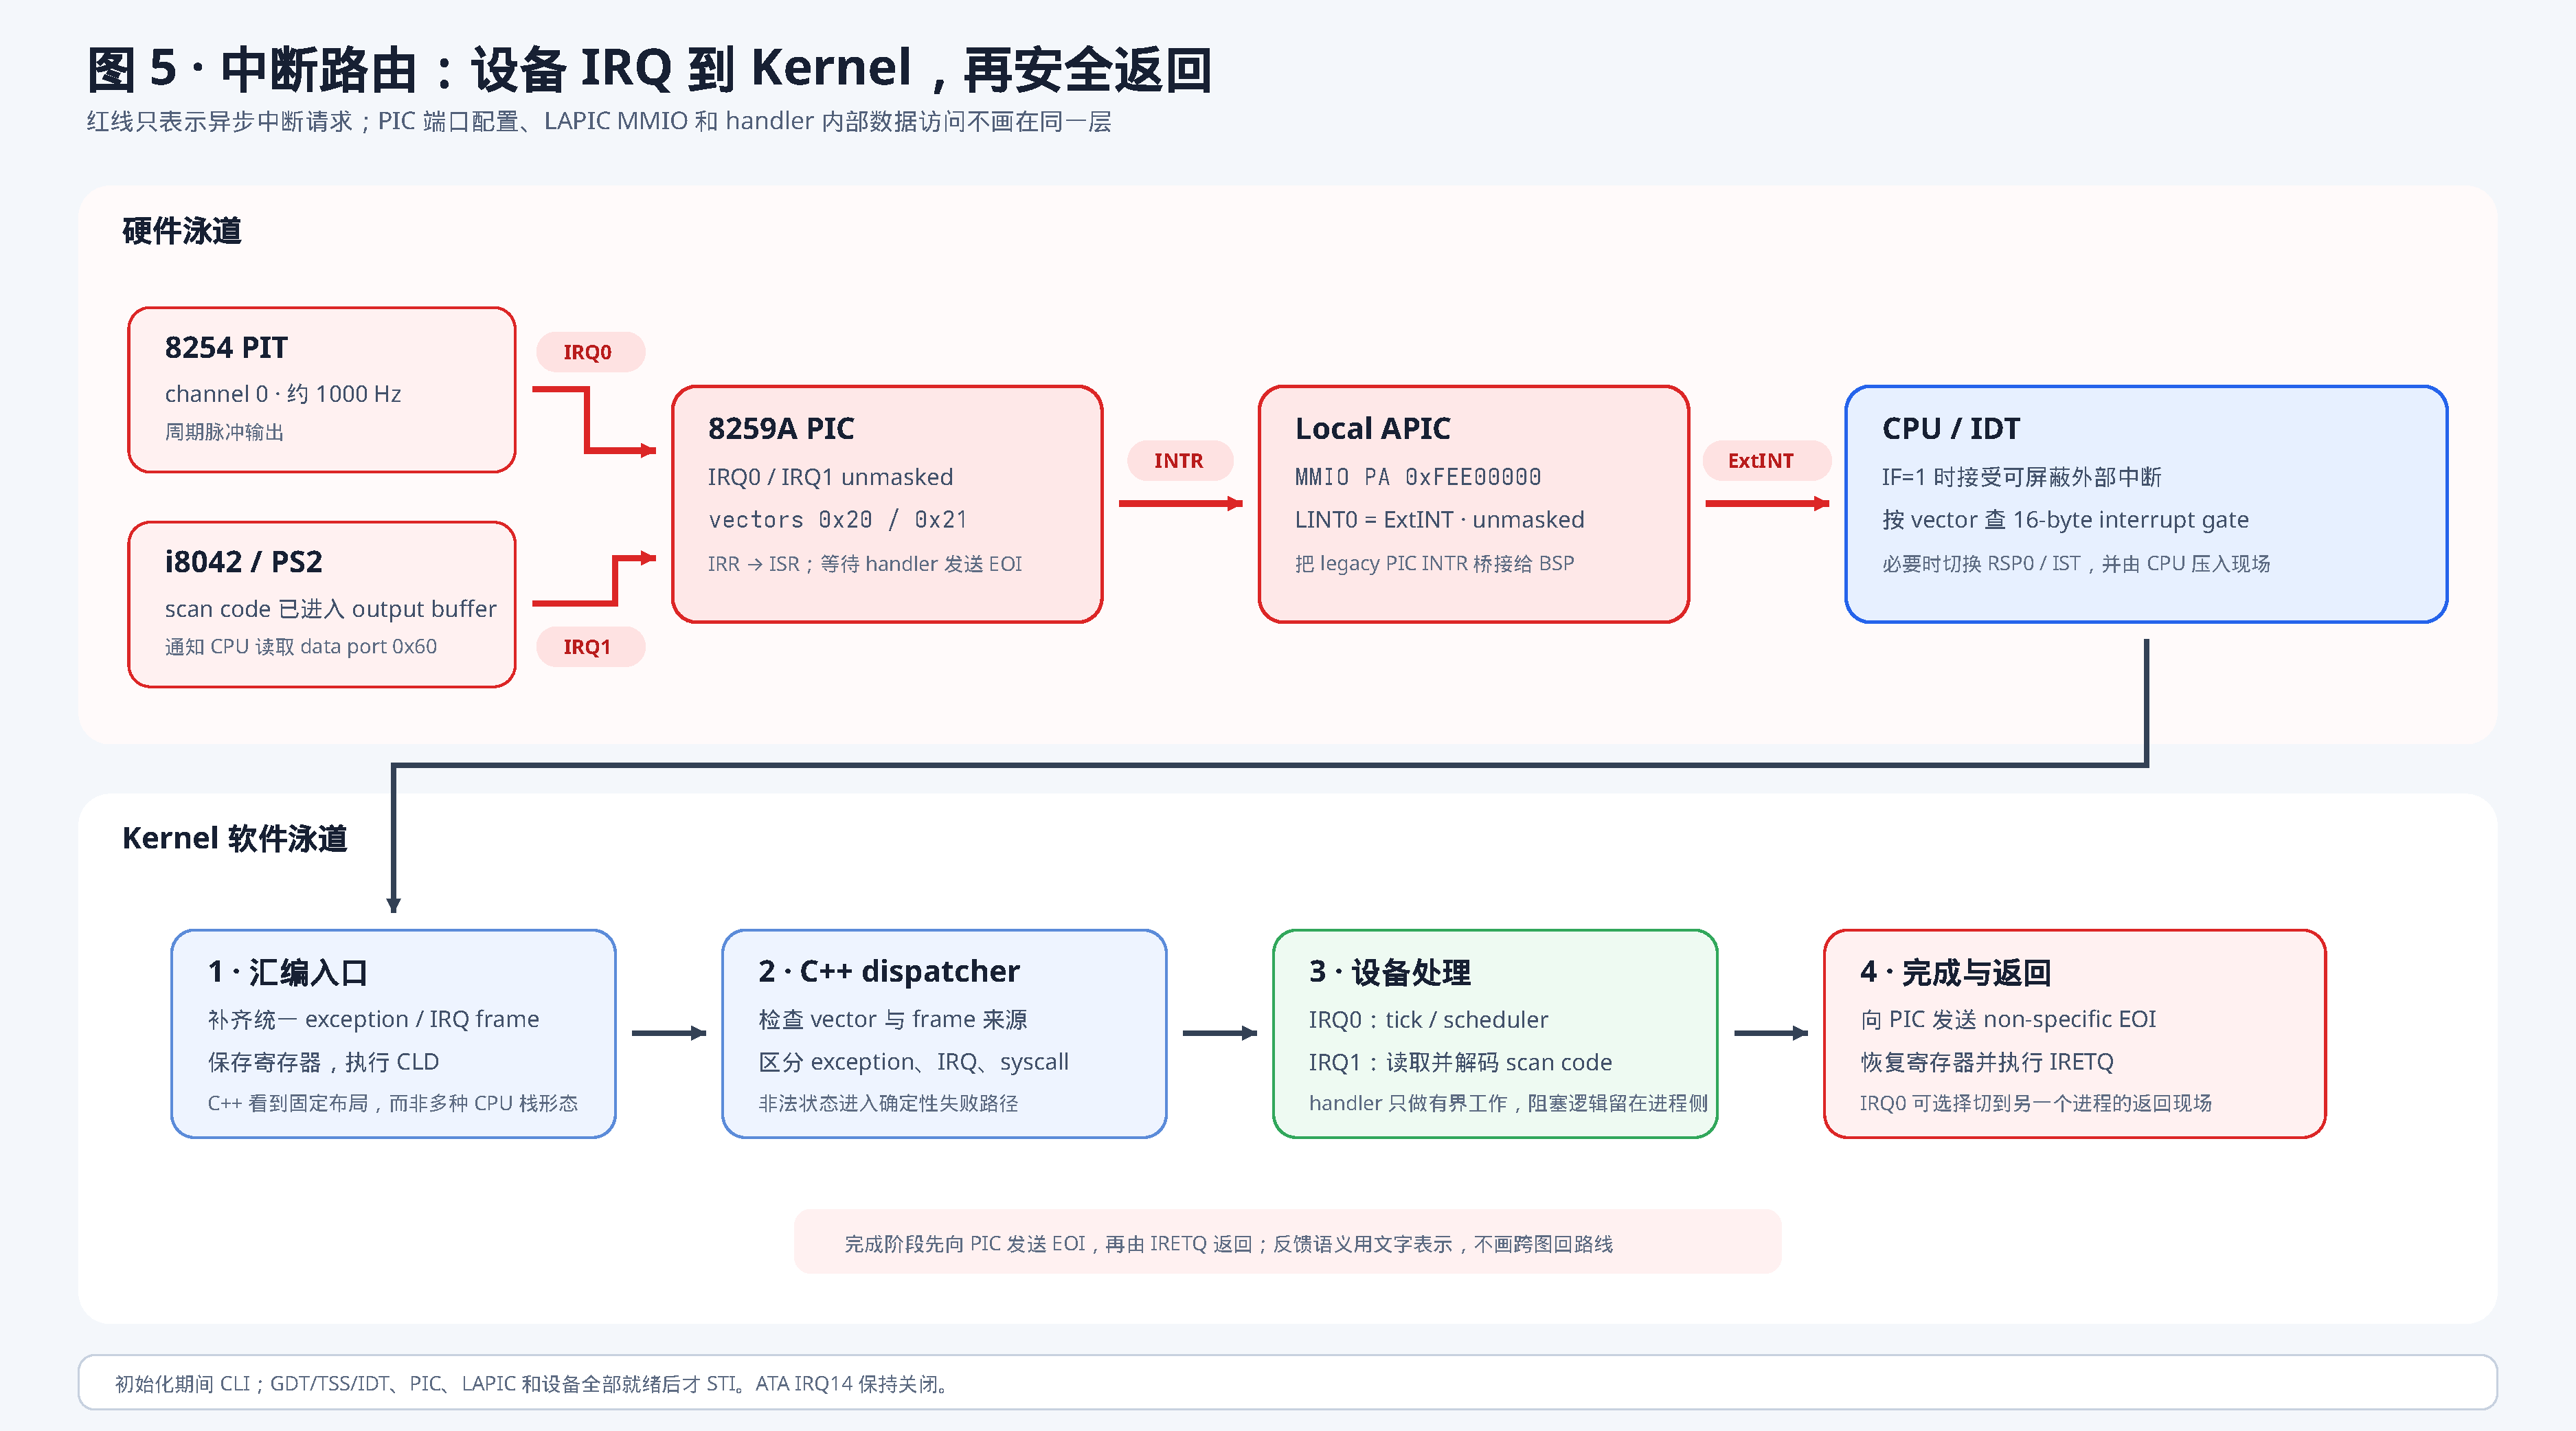
\includegraphics[width=0.96\textheight,height=0.82\textwidth,keepaspectratio]
    {figures/system_wiring/interrupt_routing.pdf}
  \caption{PIT/键盘的硬件 IRQ 经 8259A PIC 和 Local APIC 到达 CPU，再由
  汇编入口、C++ 分派、设备处理和 EOI/IRETQ 完成闭环。上半页红线是通知，
  下半页深色箭头是软件控制流，不能混成“设备直接调用 handler”。}
  \label{fig:interrupt-routing-full}
\end{sidewaysfigure}
\clearpage

\topic{一、IRQ 和 vector 为什么不是同一个编号}
\term{IRQ}{Interrupt Request，中断请求}是设备/控制器一侧的输入编号，例如
PIT 接 PIC IRQ0、键盘控制器接 IRQ1。\term{vector}{中断向量}是 CPU 用来索引
IDT 的 0--255 编号。PIC 初始化时建立映射，因此 IRQ0 可被交付为 vector
\code{0x20}，IRQ1 可被交付为 vector \code{0x21}。

必须重映射的原因是 CPU 低向量已经保留给架构异常。如果 PIC 延续早期默认范围，
设备 IRQ 会与除零、保护错误等异常编号重叠，handler 便无法仅凭 vector 判断
来源。重映射改变软件可见向量，不改变 PIT 仍连在 IRQ0 这条硬件事实。

\begin{osgridlongtable}{L{0.16\linewidth}L{0.24\linewidth}L{0.27\linewidth}L{0.23\linewidth}}
名称 & 所在层 & 本图例子 & 谁配置或产生 \\ \hline
IRQ line & 设备到中断控制器的请求 & IRQ0、IRQ1 & PIT/i8042 产生，PIC 接收 \\ \hline
PIC vector & 控制器交给 CPU 的编号 & \code{0x20}、\code{0x21} & Kernel 初始化 PIC offset \\ \hline
IDT entry & CPU 按 vector 找到的 16 B gate & entry 32、33 & Kernel 构造并 \code{lidt} \\ \hline
handler & 保存现场后运行的软件 & timer/keyboard C++ 分派 & 汇编 adapter 调用 \\ \hline
\end{osgridlongtable}

\topic{2.1 PIT 和 i8042 先保存各自的事件事实}
PIT channel 0 到期时产生周期脉冲；i8042 在 output buffer 已有扫描码时产生
IRQ1。红线只携带“请处理”的请求，不携带 tick 数字或扫描码字节。timer handler
通过已知设备语义增加软件 tick；keyboard handler 还必须从 port
\code{0x60} 读取控制器保存的数据。

\topic{2.2 PIC 仲裁、记录并等待 EOI}
PIC 的 IRR 记录待处理请求，IMR 决定哪些输入被屏蔽，ISR 记录已经交付但尚未
完成的请求。它按优先级选择 IRQ，输出 INTR。CPU 接受并应答后，PIC 提供
映射后的向量。handler 完成时发送 EOI，PIC 才能从 in-service 状态释放对应
层级。

EOI 太早可能让同源事件在共享状态尚未稳定时重入；EOI 太晚或遗漏则可能阻塞
后续中断。级联从片 IRQ 还涉及从片和主片的正确确认顺序。本项目当前只放行
主片 IRQ0/IRQ1，但驱动仍明确遵循完成协议。

\topic{2.3 Local APIC virtual-wire 是兼容桥}
Local APIC 位于 CPU 一侧，LINT0 配成 ExtINT 后，可把 legacy PIC 的 INTR
桥接给 BSP。这条路径叫 virtual wire，不表示它是“假的中断”；它是现代 APIC
体系承接传统 PIC 的兼容模式。Local APIC 自身通过 MMIO 配置，不在 Port I/O
图的蓝色总线上。

\topic{2.4 CPU 还要经过四道接收条件}
普通可屏蔽中断到达 handler，至少需要：

\begin{enumerate}[leftmargin=2.2em]
  \item 设备启用对应事件并真正提出 IRQ；
  \item PIC 没有在 IMR 屏蔽该输入，且路由/级联状态有效；
  \item Local APIC 的 LINT0/ExtINT 路径有效；
  \item CPU 的 RFLAGS.IF 为 1，IDT 对应 gate present 且入口可执行。
\end{enumerate}

所以“执行过 \code{sti}”不是完整证明。任何上游门关闭都不会进入 handler；
反过来，异常和 NMI 另有规则，也不会因为 IF 清零而全部消失。

\topic{三、CPU/IDT 如何安全改变控制流}
\term{IDT gate}{中断描述符表门}给出目标代码段、入口偏移、gate 类型、DPL、
present 位和可选 IST 编号。CPU 接受事件后按规范保存返回现场；跨特权级时
还要切到 TSS.RSP0 或指定 IST 栈。这个过程由硬件约束，设备不能任意指定内核
函数指针。

本项目的汇编入口把“CPU 有时压 error code、有时不压”的不同异常/IRQ 形态
规范成固定 C++ 可读 frame，保存 15 个通用寄存器并执行 \code{cld}。调用
C++ 前还要满足 System V AMD64 栈对齐。handler 看到的是经 adapter 明确定义的
数据结构，不是可以随意改字段顺序的普通函数参数。

\topic{四、Kernel 软件泳道的四个提交点}\par
\begin{osgridlongtable}{L{0.16\linewidth}L{0.27\linewidth}L{0.30\linewidth}L{0.17\linewidth}}
阶段 & 必须完成 & 失败边界 & 提交证据 \\ \hline
汇编入口 & 保存/规范化现场，建立 ABI 栈 & 任何调用前，不可破坏原现场 & 固定 frame 可审计 \\ \hline
C++ dispatcher & 检查 vector、来源与当前上下文 & 未知/非法状态走确定性失败 & 选中唯一 handler \\ \hline
设备处理 & 读取事实，更新最小有界状态 & 不在 IRQ 中无限等待或做阻塞用户工作 & tick/扫描码入队 \\ \hline
完成返回 & 按来源发送 EOI，恢复现场，\code{iretq} & 不得返回失效进程/栈 & 下一现场继续执行 \\ \hline
\end{osgridlongtable}

IRQ0 可能在返回时切换到另一个进程的保存现场，因此“返回”不一定回到被打断
进程；但无论选择哪个现场，都必须具有正确 CR3、Ring 0 栈、用户 frame 与资源
所有权。调度决定属于内核策略，IRETQ 只按给定合法现场执行硬件恢复。

\begin{sidewaysfigure}[p]
  \centering
  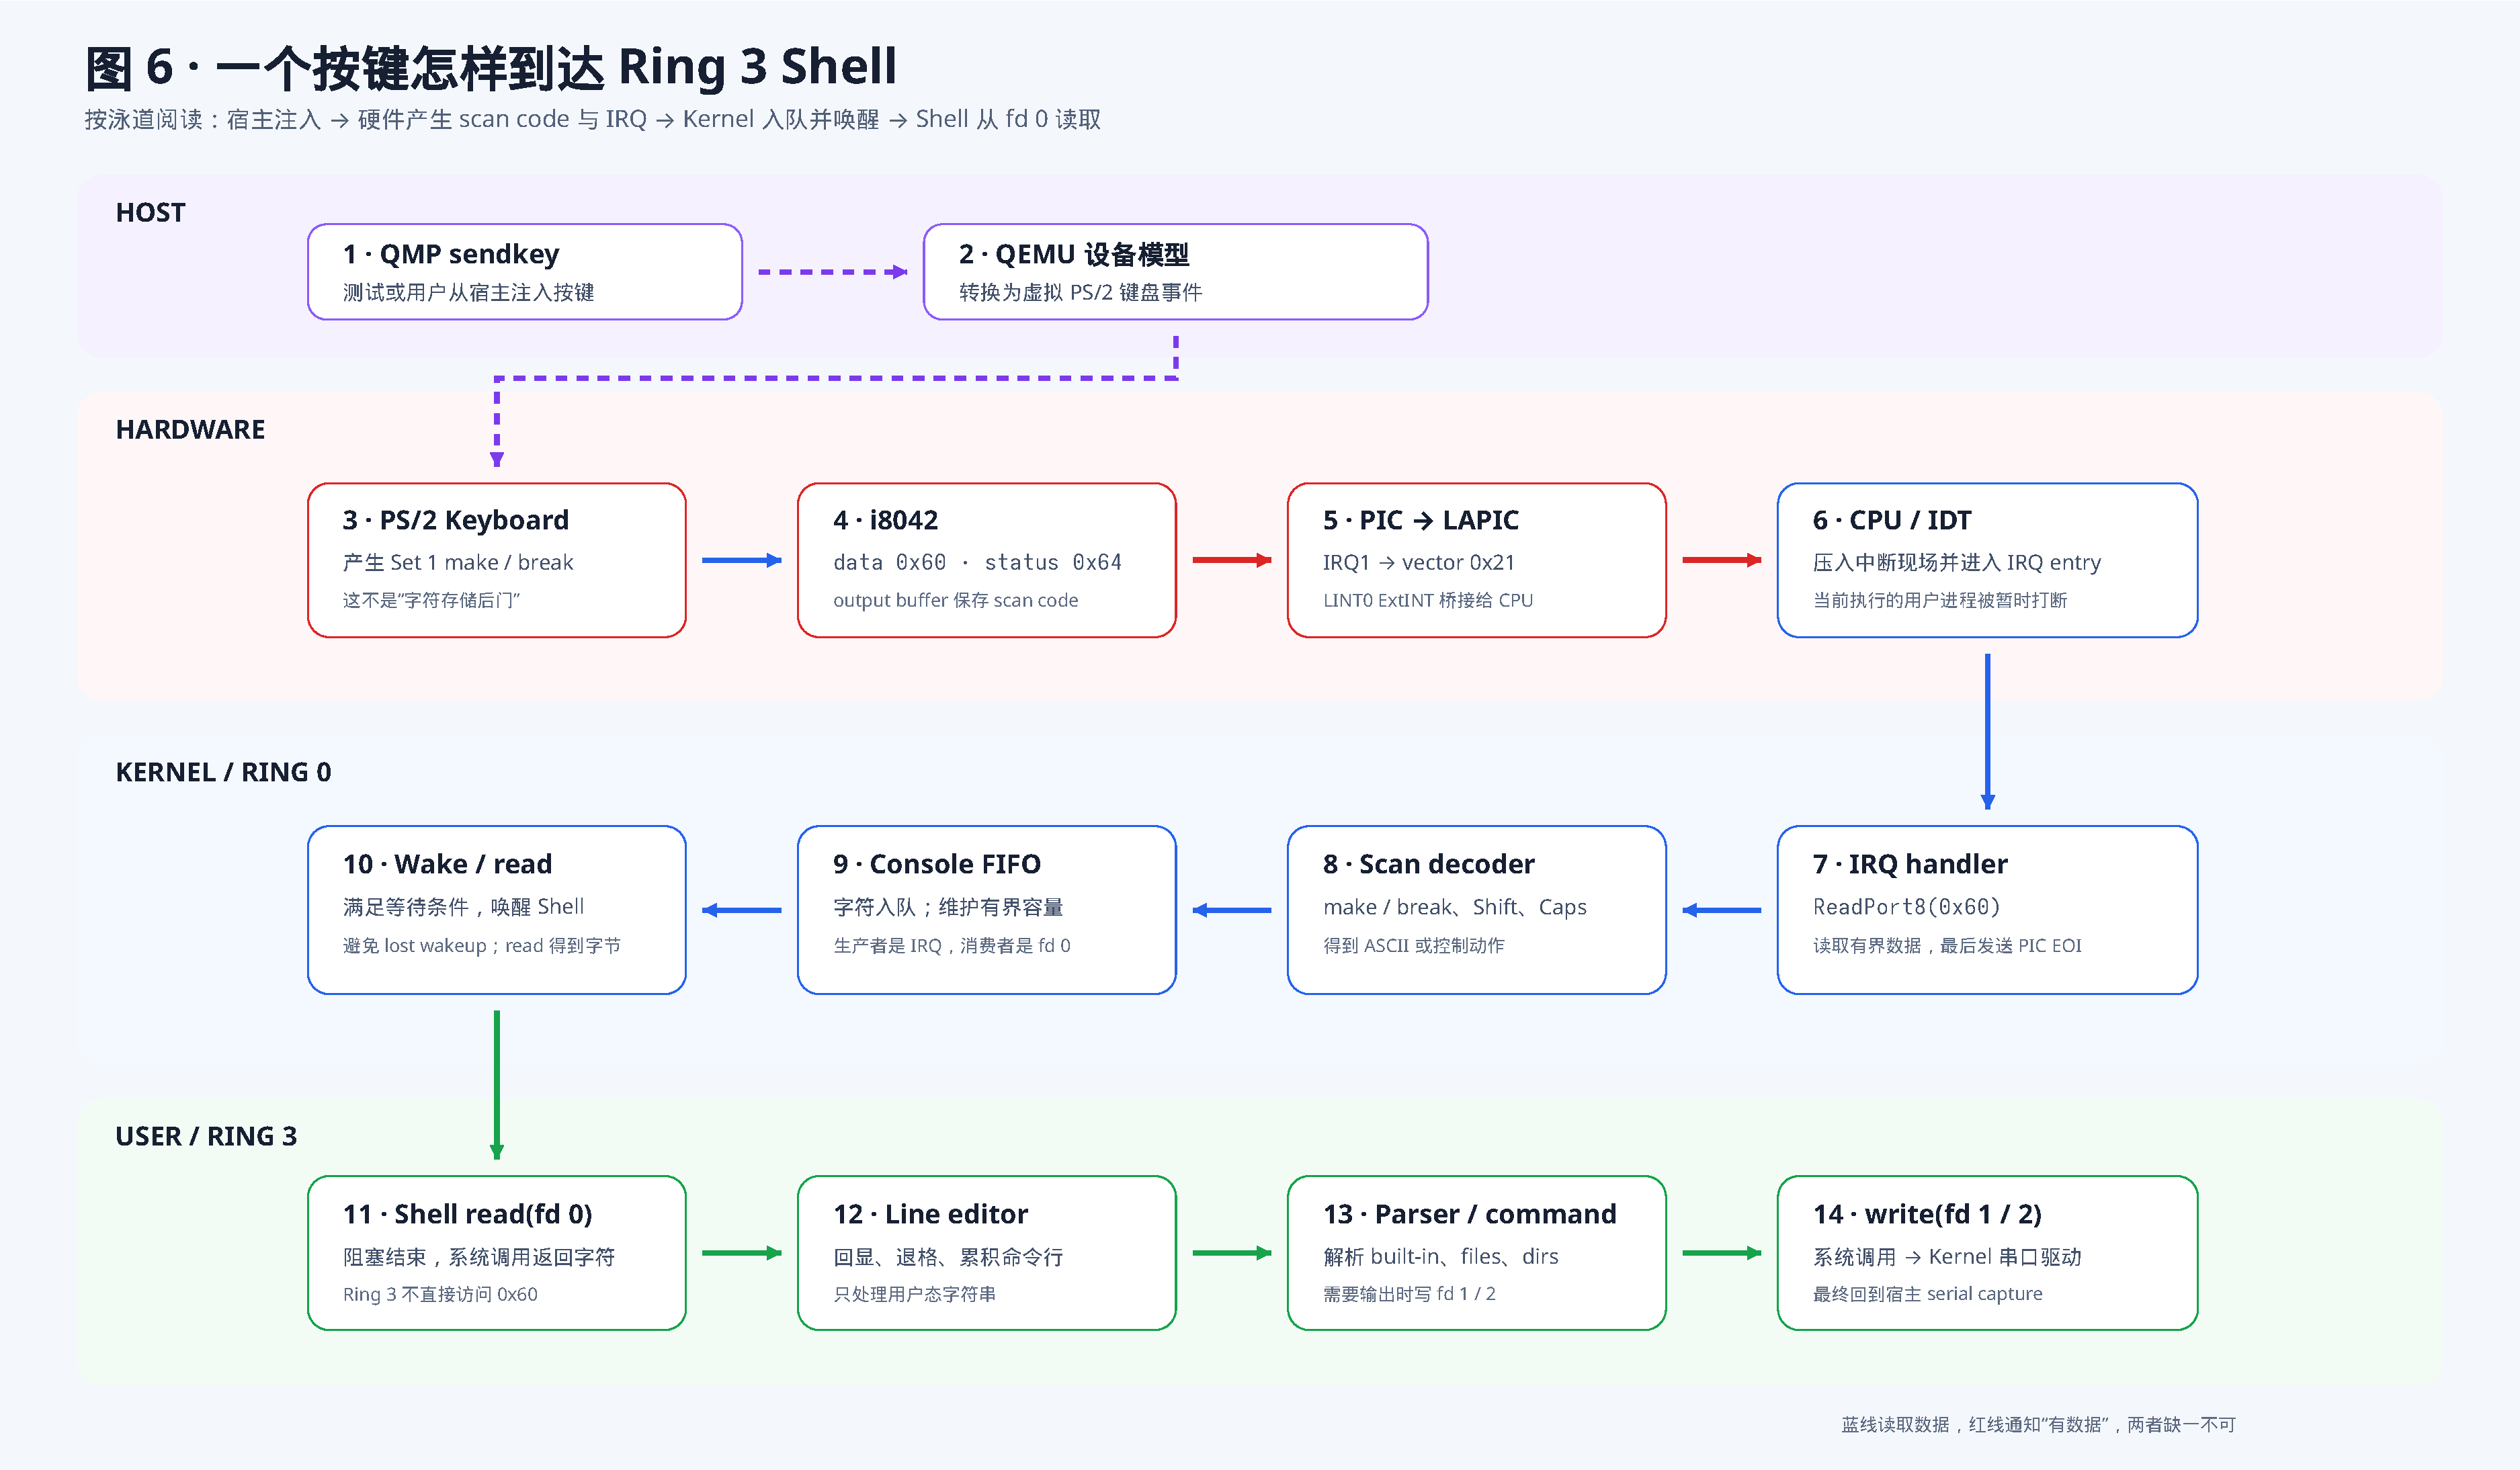
\includegraphics[width=0.96\textheight,height=0.82\textwidth,keepaspectratio]
    {figures/system_wiring/keyboard_to_shell.pdf}
  \caption{一个按键从宿主 QMP、QEMU PS/2 设备、IRQ1、Kernel FIFO 到 Ring 3
  Shell 的十四步路径。紫线是宿主注入，红线是 IRQ 通知，蓝线是内核数据流，
  绿线是用户态处理；不同颜色的箭头不可互换。}
  \label{fig:keyboard-to-shell-full}
\end{sidewaysfigure}
\clearpage

\topic{5.1 步骤 1--2：宿主请求不等于 Guest 字符}
自动化测试通过 QMP \code{sendkey} 向 QEMU 提交按键动作。QEMU 设备模型把它
转换成虚拟 PS/2 键盘事件。宿主传入的是控制命令，不是直接写入 Ring 3
缓冲区；QMP 与 Guest 的内存、端口和系统调用没有共用函数调用栈。

\topic{5.2 步骤 3--4：键盘产生扫描码，i8042 保存字节}
PS/2 键盘产生 Set 1 make/break 序列。i8042 把扫描码放进 output buffer，
状态端口 \code{0x64} 报告可读，数据端口 \code{0x60} 返回字节。按下 A 与
松开 A 是不同序列；Shift/Caps 状态也必须由后续解码器记忆，不能把每个字节
直接强制转换为 ASCII。

\topic{5.3 步骤 5--7：通知抵达，handler 才读取数据}
IRQ1 经 PIC 和 Local APIC 变成 vector \code{0x21}。CPU 保存现场并进入
IRQ entry；handler 再检查 i8042 状态并读取 \code{0x60}。顺序不能反过来：
没有读取数据寄存器，IRQ 线本身不会告诉 handler 是哪个键；没有正确中断路由，
缓冲区即使有数据也不会异步唤醒软件。

\topic{5.4 步骤 8--10：扫描码成为有界字符队列}
scan decoder 组合 make/break、扩展前缀、Shift 和 Caps 状态，产出字符或控制
动作。ConsoleInput 使用固定容量 FIFO 保存结果；生产者是 IRQ 路径，消费者是
等待 fd 0 的进程。队列满时必须遵守明确丢弃/计数策略，不能越界写；由空变为
可读时唤醒满足条件的 waiter，不能无条件唤醒所有进程。

\term{lost wakeup}{丢失唤醒}发生在“检查为空”和“登记睡眠”之间若没有同一
受保护事务：数据可能恰在缝隙到达，生产者看不到 waiter，消费者随后永久睡眠。
本项目把 compare-and-block 与队列状态放进明确锁/调度协议，Shell 的 read
才不会偶发卡死。

\topic{5.5 步骤 11--14：系统调用把字符交给 Shell}
Shell 在 Ring 3 对 fd 0 发起 read。系统调用验证用户缓冲区、解析当前进程
FileTable、确认对象可读；无数据则按协议阻塞，有数据则从 FIFO 复制到用户页。
Ring 3 从不直接执行 \code{in 0x60}，否则会绕过设备所有权、并发和隔离。

line editor 处理回显、退格和行边界，parser 把整行分成命令与参数，built-in
再访问文件/目录。输出经 fd 1/2 回到 Kernel 串口对象，最终进入宿主 serial
capture。因此输入和输出是两条独立端到端路径，在 Shell 层才汇合。

\topic{六、怎样按症状定位断在哪一层}\par
\begin{osgridlongtable}{L{0.25\linewidth}L{0.30\linewidth}L{0.35\linewidth}}
现象 & 首先检查 & 原因 \\ \hline
QMP 成功但没有 IRQ1 & QEMU 设备选择、i8042 初始化、PIC IMR、LAPIC、IF & 宿主命令只证明注入请求被接受 \\ \hline
IRQ1 计数增加但无字符 & \code{0x64} 状态、\code{0x60} 读取、扫描码 decoder & 通知路径正常不等于数据解释正常 \\ \hline
字符入 FIFO 但 Shell 卡住 & waiter 登记、唤醒条件、调度、fd 0 对象 & 硬件路径已完成，故障位于阻塞协议 \\ \hline
Shell 收到错字符 & make/break、扩展前缀、Shift/Caps 状态 & 不能只检查 IRQ 数量 \\ \hline
能输入但无回显 & fd 1/2、系统调用返回、UART THRE 与 serial capture & 输出链独立于输入链 \\ \hline
第一个键后再无中断 & i8042 数据是否取走、PIC EOI 是否发送 & 设备/PIC 可能仍保持未完成状态 \\ \hline
\end{osgridlongtable}

\begin{failurebox}
中断 handler 的日志本身会改变时序，串口轮询甚至可能显著延长关中断窗口。
调试时先用计数器、固定标记和超时证明边界，热路径成功后移除逐事件日志；
最终证据应同时覆盖 IRQ 到达、数据守恒、无丢失唤醒、正确 EOI 和合法返回现场。
\end{failurebox}

